\chapter{Experiments and Results}


\section{Experiments}

\iffalse
SVM-Regression
Random-Forest Regression
Deep Learning Network

Neural Net Sequence Embeddings
One-Hot Encodings
Modfied n-grams skip-grams
\fi

The focus of the experiments are concentrated on the properties of protein as they have complex structures. The binding of protein and drug depend on various attributes of protein like acidity, hydrophobicity, binding pockets etc and the structure of drug. The attributes are quite closely related to primary and secondary structure of protein themselves. Therefore, our model aims to relate all these multiple components with matrix representation and confirming to Figure ~\ref{fig:kiba_drug_protein} prediction.

\subsection{Features Selection}
\subsubsection{Primary Feature Selection}
The sequence information of drugs and proteins live in their canonical form. Exploring to the other embedding technique used in language theory, the modified N-Grams Skip-Grams (m-NGSG) was supposed to undertake the mutational agreements when the proteins and drug interaction was brought in question. However, it fared quite badly than the Neural Net Sequence Embeddings. Mostly the issue can be related to that if the algorithm misses the tight relationship among the amino-acid neighborhood, then the protein with different structure may seem to act similarly: a strong disagreement on principle that certain proteins with slight modification on the sequence have different functional and chemical properties. It could still be used for Poisson-Hidden Markov Model for some other properties, but primary encodings can't be relied on m-NGSG. 

Therefore we relied on Neural Net Sequence Embedding technique to form the primary representation. Both protein and drug were converted to Embedding vectors after creating their one-hot encoding.

\subsubsection{Secondary Features Selection}
These are the structural components of protein especially related to alpha and beta strands of Protein segments. All the protein Sequences are subjected to Equation~(\ref{eq:pssm}) from the one-hot encodings. The \acrshort{pssm} matrix is calculated using PSI-BLAST\cite{Schaffer2001}. Then all the testing protein sets are evaluated with the resultant PSSM to form a new PSSM matrix specific to the testing protein. Thus, we expect to explore how proteins relate with the interaction experiments with the protein domain. From the \acrshort{pssm}, we evaluate the other evolutionary and distance vectors using equations \ref{eq:rpt}, \ref{eq:pssmddt}, \ref{eq:pssmsdt} and \ref{eq:edt}.

\subsection{Implementation}
% We explore basically the following algorithms for analyses on protein-drug interactions:

\subsubsection{Stacked Features, LSTM Network}
Basically, we implement the ~\ref{fig:dlm} for our model design. It is implemented in Python using the TensorFlow framework consisting of keras. The training contained of 100 epochs and required full 4 complete days to complete the training in quad-core processor. The training and testing was done in a 5-fold cross-validation set prepared manually. To evaluate the performance of the model, we used concordance index(CI)\cite{Xu2015} as defined by equation~\ref{eq:ci}:
\begin{equation}
    CI = \frac{1}{Z} \sum_{\delta_i > \delta_j} h(b_i - b_j)
    \label{eq:ci}
\end{equation}
where $b_i$ is the prediction value for higher affinity $\delta_i$ and $b_j$ is the prediction value for smallery affinity $\delta_j$, $Z$ is the normalization constant and $h(m)$ is the unit step function:
\begin{equation} h(x) = 
    \begin{cases}
        1,& \quad {if x>0} \\
        0.5, & \quad{ if x=0 } \\
        0, & \quad{if x<0} \\
    \end{cases}
\end{equation}

\section{Results}
The training of the model proved a better choice as we placed a LSTM layer to get a generalization of all the feature sets extracted from the drug and protein sequence. In a primordial network, the c-index rised from 70\% to 75\% simply between the choice of Dense Layer and LSTM Layer. 

The validation loss and the cindex scores(equation~\ref{eq:ci}) were 16\% and 89\% respectively when we used our full model. The plot of ~\acrshort{kiba} prediction scores and the actual scores for training sets is shown in Figure ~\ref{fig:pred_train}
\begin{figure}[ht]
    \subfigure[Training Actual Scores]{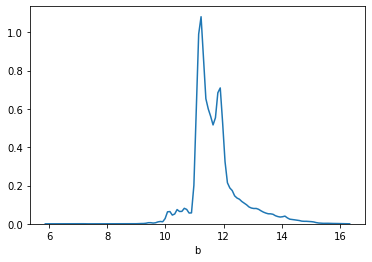
\includegraphics[width=.3\textwidth]{mainmatter/4-Results/images/train_y.png}}
    \subfigure[Training Predicted Scores]{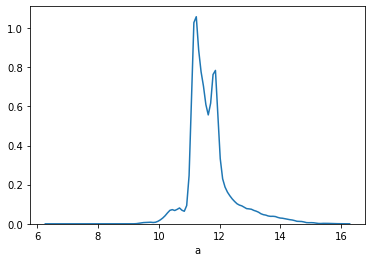
\includegraphics[width=.3\textwidth]{mainmatter/4-Results/images/pred_train_y.png}}
    \subfigure[Training Scores Difference]{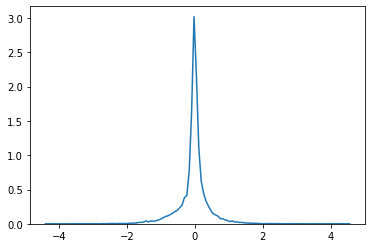
\includegraphics[width=.3\textwidth]{mainmatter/4-Results/images/train_diff.png}}
    \caption{Training Results based on KIBA Score Prediction}
    \label{fig:pred_train}
\end{figure}

Similarly, the prediction scores and actual scores for validation sets is shown in Figure ~\ref{fig:val_train}
\begin{figure}[ht]
    \subfigure[Testing Actual Scores]{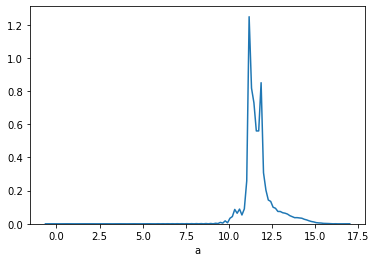
\includegraphics[width=.3\textwidth]{mainmatter/4-Results/images/val_y.png}}
    \subfigure[Testing Predicted Scores]{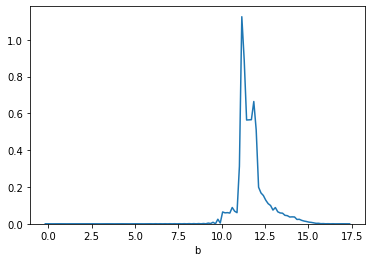
\includegraphics[width=.3\textwidth]{mainmatter/4-Results/images/pred_val_y.png}}
    \subfigure[Testing Scores Difference]{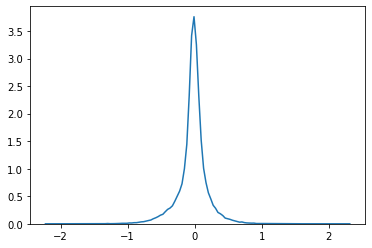
\includegraphics[width=.3\textwidth]{mainmatter/4-Results/images/val_difference.png}}
    \caption{Testing Results on KIBA score Prediction}
    \label{fig:val_train}
\end{figure}

\iffalse The similarity measures are evaluated using \cite{Cock2009}. \fi

\iffalse
The accuracy plots and cindex plots are shown in Figure ~\ref{fig:results}
\begin{figure}
    
\end{figure}
\fi